\section{Object detection Results}
\label{sec:objectDetectionResults}

The first approach is to train object detection models.
For this, the \ac{YOLO}v7 and the \ac{GELAN}-c and \ac{GELAN}-e model versions from \ac{YOLO}v9 are trained.
After conducting a large number of experiments with different models and versions of datasets, the best results are obtained.
The best performance scores are obtained from an experiment conducted with the \ac{GELAN}-e model which outperformed the other models in accuracy.
These results are acquired by fine-tuning a model, which is pre-trained on the COCO dataset.
The onlySwitchesLeftRight sub-dataset from RailSem19 is used to train the model (\autoref{sec:usedDatasetsYOLOs}).
\autoref{fig:objectDetectionResultsMetrics} shows performance graphs like the F1 Curve and the Precision-Recall Curve, as well as the confusion matrix with both classes.

\vspace{0.5cm}

\begin{figure}[H]
    \centering
    \begin{subfigure}{0.32\textwidth}
        \centering
        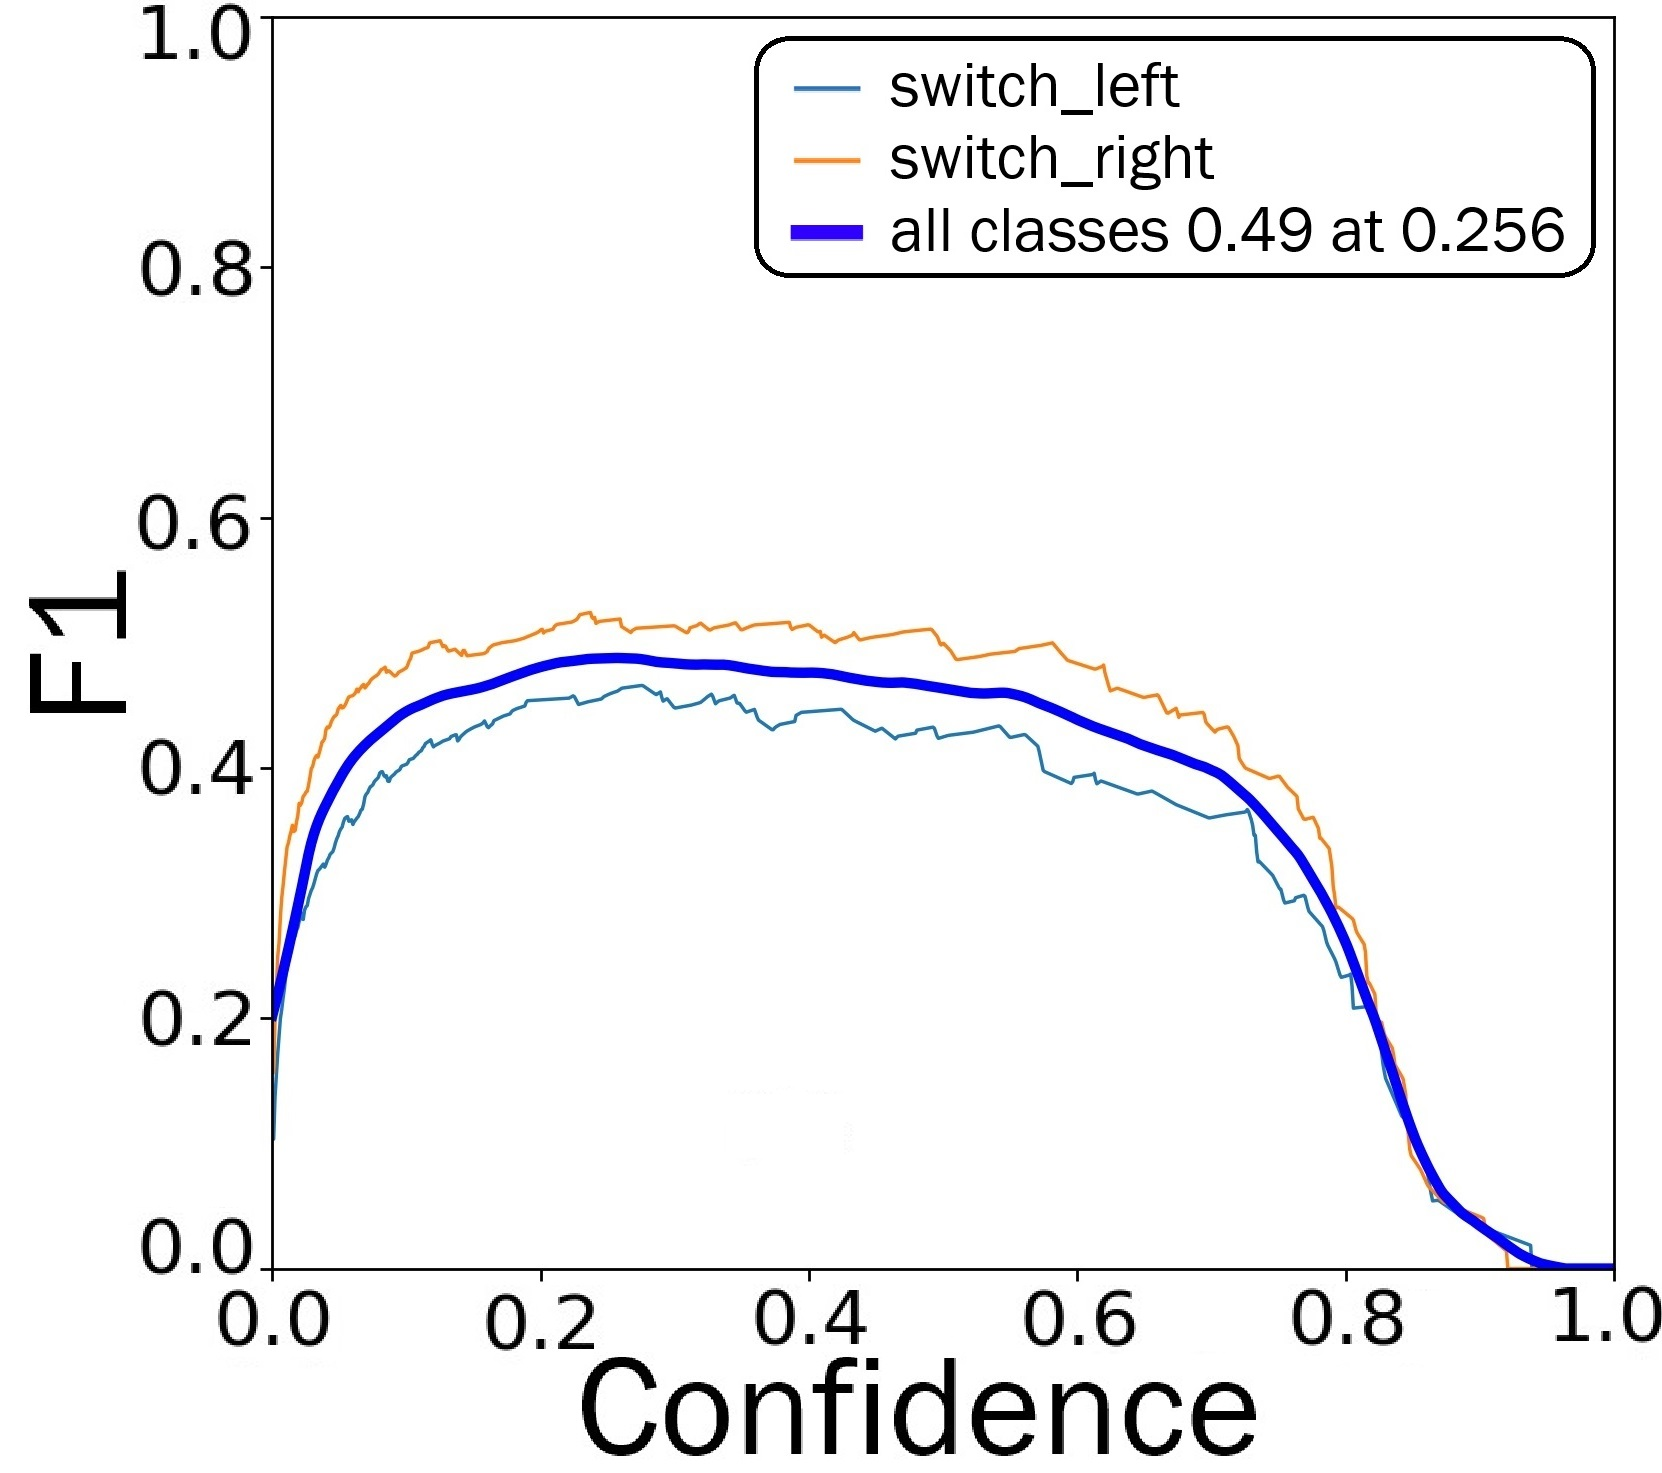
\includegraphics[width=\linewidth,height=4.5cm,keepaspectratio]{PICs/experiments/objectdetectionExperiment/F1_curve_updated_v2.jpg}
        \caption{F1-Confidence Curve}
        \label{fig:objectDetectionResultsMetrics_a}
    \end{subfigure}
    %\hspace*{0.02\textwidth} % Abstand manuell steuern
    \begin{subfigure}{0.32\textwidth}
        \centering
        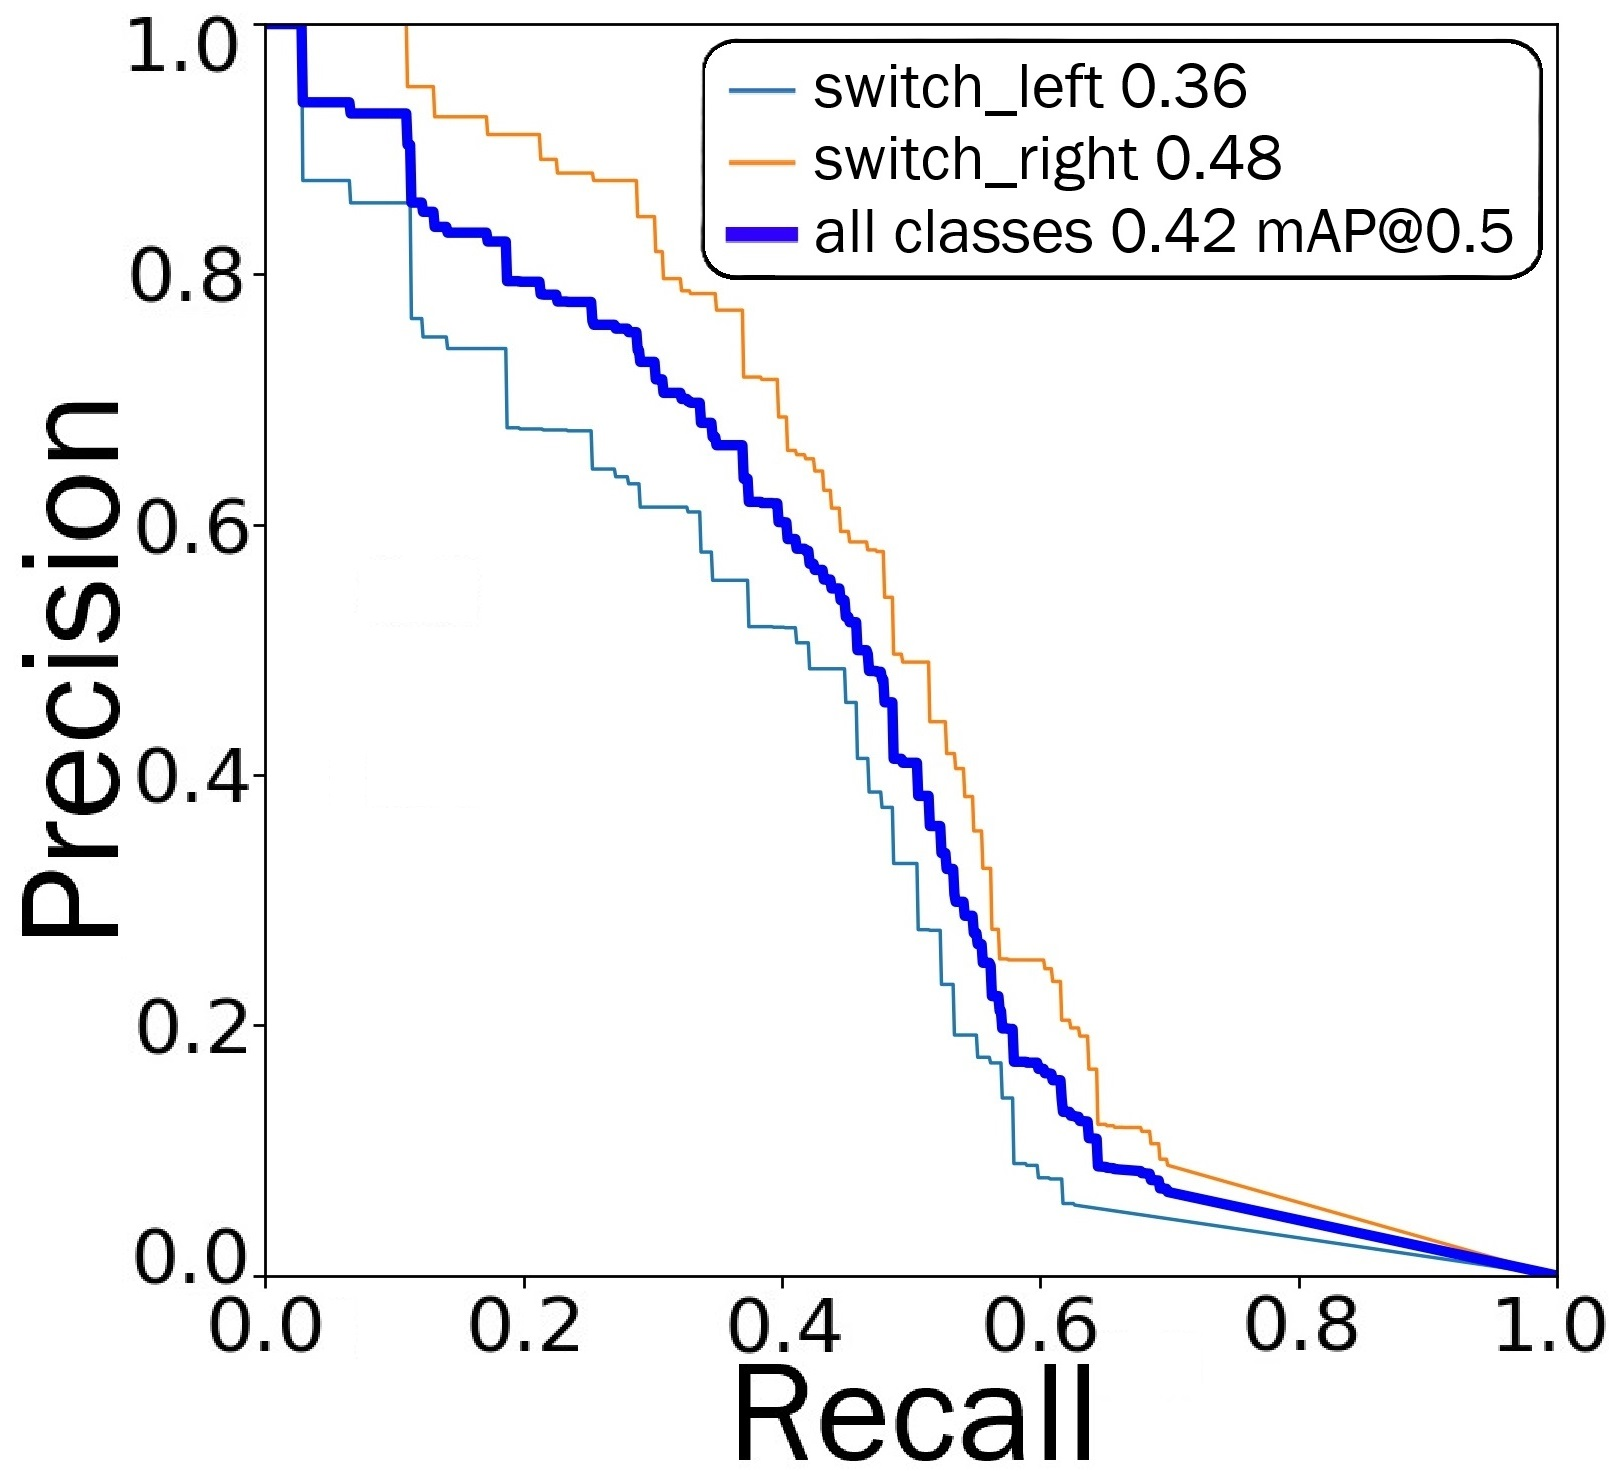
\includegraphics[width=\linewidth,height=4.5cm,keepaspectratio]{PICs/experiments/objectdetectionExperiment/PR_curve_updated_v2.jpg}
        \caption{Precision-Recall Curve}
        \label{fig:objectDetectionResultsMetrics_b}
    \end{subfigure}
    %\hspace*{0.02\textwidth} % Abstand manuell steuern
    \begin{subfigure}{0.32\textwidth}
        \centering
        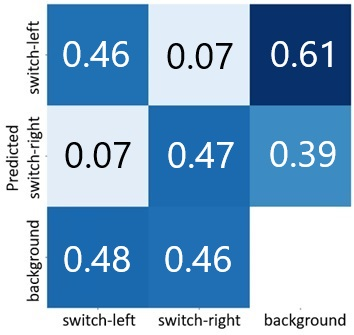
\includegraphics[width=\linewidth,height=4.5cm,keepaspectratio]{PICs/experiments/objectdetectionExperiment/confusion_matrix_updated_v2.jpg}
        \caption{Confusion Matrix}
        \label{fig:objectDetectionResultsMetrics_c}
    \end{subfigure}
    \caption{Results of best-performing object detection model experiment: \ac{GELAN}-e fine-tuned on onlySwitchesLeftRight and pre-trained on COCO.
    Thin Orange lines are $switch\_right$ labels, thin blue lines are $switch\_left$ labels and thick blue lines are all classes}
    \label{fig:objectDetectionResultsMetrics}
\end{figure}

\noindent However, as visualized in \autoref{fig:objectDetectionResultsMetrics} the Precision-Recall Curve and the F1 Curve show unsatisfying results.
The confusion matrix also indicates that the model's prediction performances are below 50\% for both classes.
The reason for that presumably lies in the complexity of the task.
Switches look similar to rails and predicting switch states further increases the difficulty, because the only difference is the start of the switch.
Additionally, the \ac{GT} bounding boxes of most switch labels are very small.
As shown in \autoref{fig:annotationAnalysis} most crops have widths of about 0.02 and heights of about 0.015 relative to the dataset images.
Converted into pixels with the image resolution of $1920 \times 1080$, this results in crops with heights of around 22 pixels and widths of around 29 pixels.
RailSem19 \cite{railsem19dataset} also states that this task is difficult.
In one of their experiments, they only considered the crops of $switch\_left$ and $switch\_right$ labels and turned it into a classification task.
Even after they expanded the crops vertically by 125\% and horizontally by 30\% to increase the context, they had many images with dimensions below 28 pixels.
After dropping those and training a denseNet161, the accuracy only achieved 67\%.

\begin{figure}[H]
    \centering
    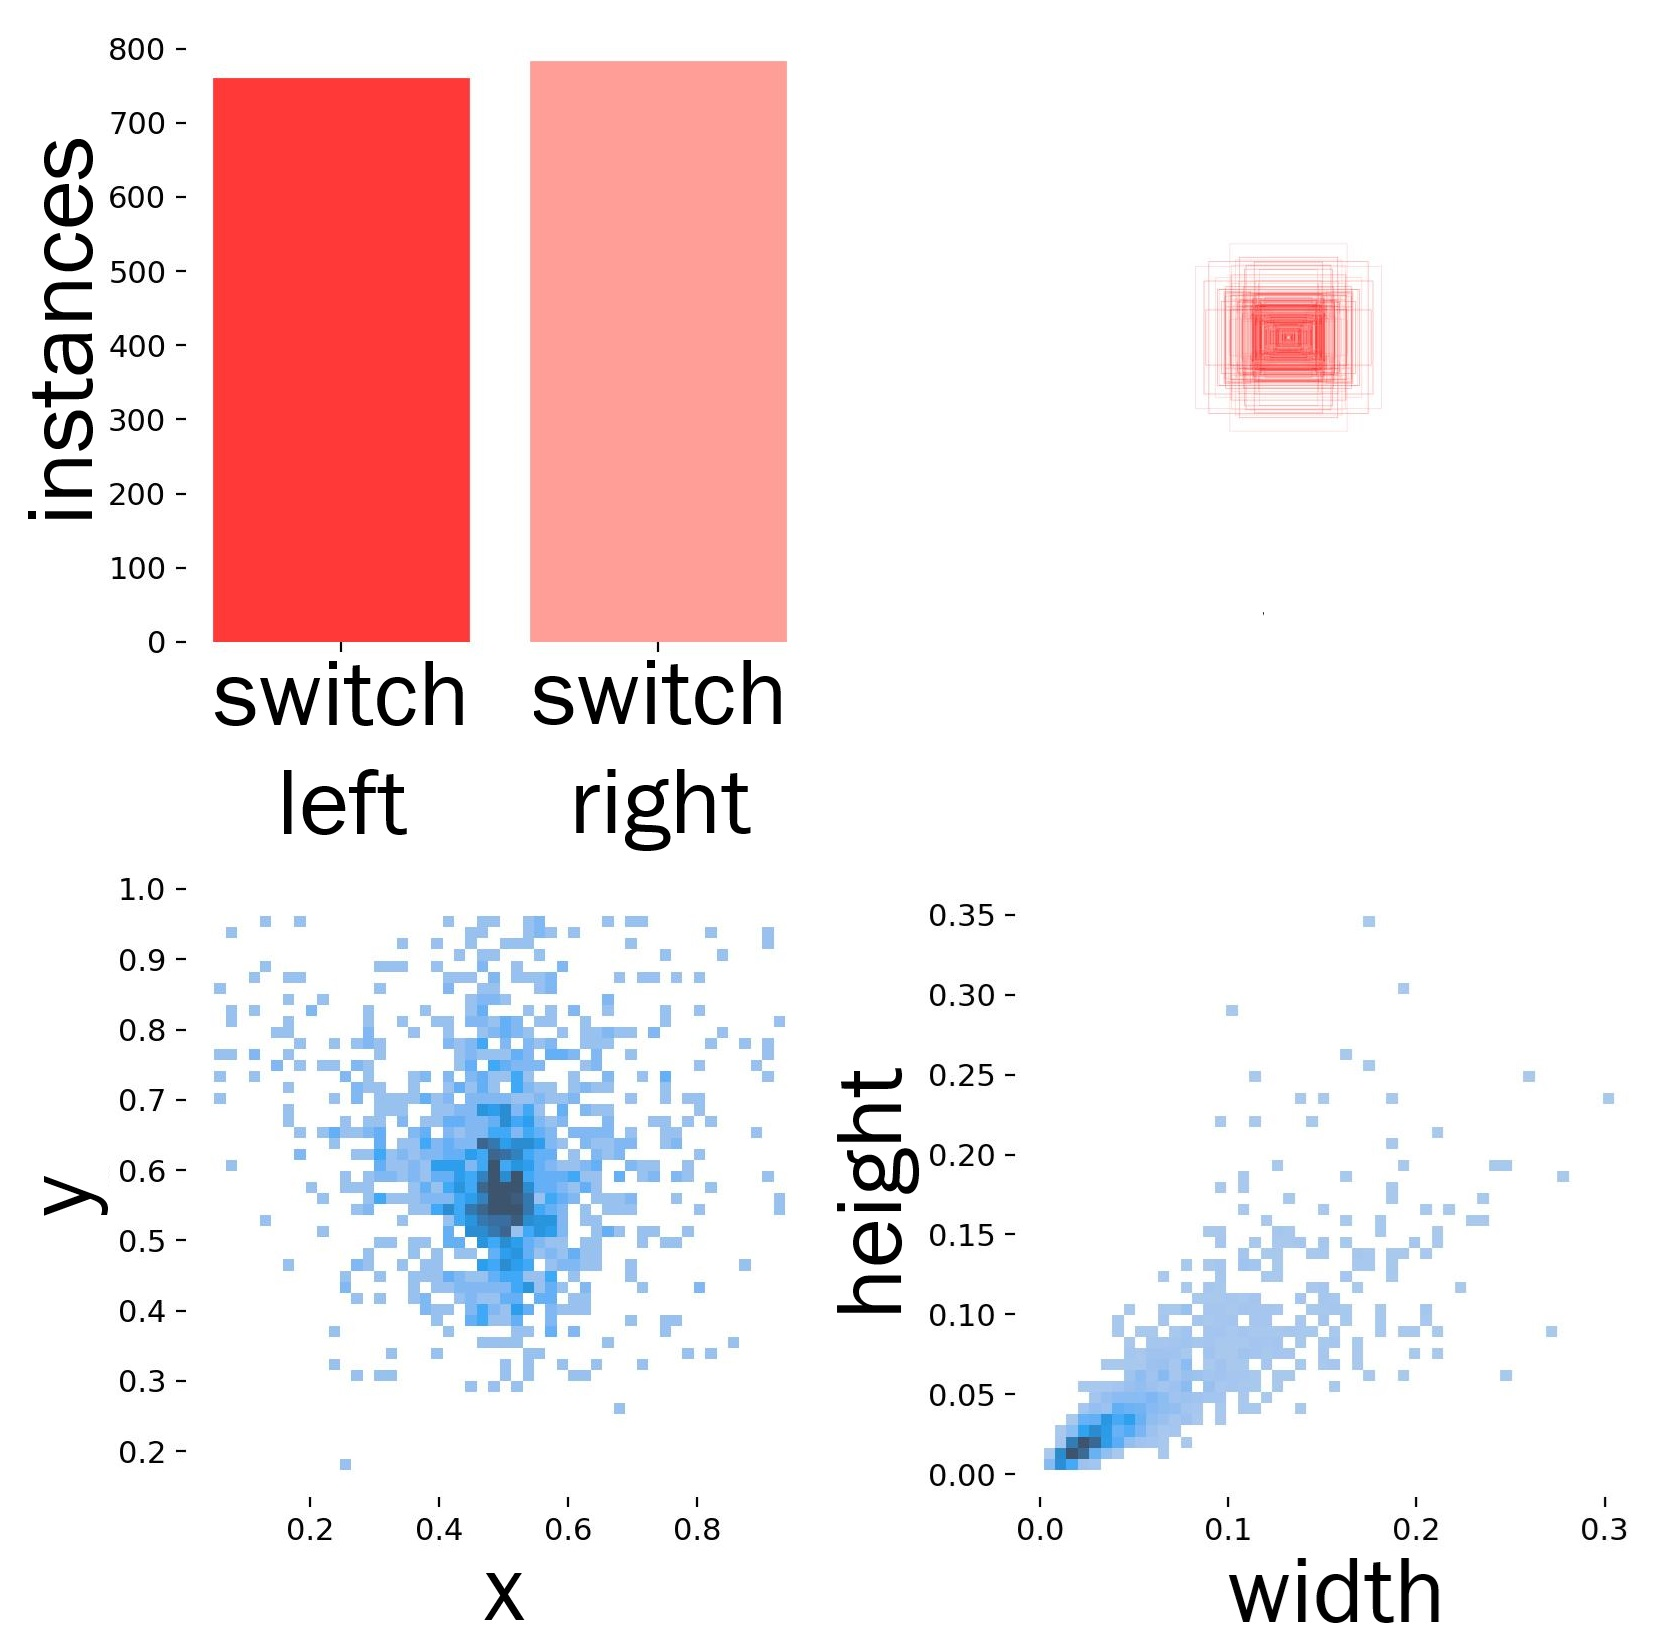
\includegraphics[width=0.6\linewidth]{PICs/experiments/objectdetectionExperiment/labels_updated.jpg}
    \caption{Annotation analyses of \ac{YOLO}v9 \cite{YOLOv9GitHub}. In the lower two graphs, the axes are relative to the image dimensions.}
    \label{fig:annotationAnalysis}
\end{figure}

\noindent Because of the complexity of this task and the unsatisfactory results it cannot be assumed switch states are correctly predicted.
Therefore the approach of predicting the direction of the train with an object detection model is discarded.
A fundamentally different approach must be found, making further experiments with semantic segmentation models unnecessary.